\chapter{Functors and natural transformations}
\label{ch:functors}
Functors are maps between categories; natural transformations are maps between functors.

\section{Many examples of functors}
\prototype{Forgetful functors; fundamental groups; $\bullet^\vee$.}
Here's the point of a functor:
\begin{moral}
	Pretty much any time you make an object out of another object,
	you get a functor.
\end{moral}
Before I give you a formal definition, let me list (informally) some examples.
(You'll notice some of them have opposite categories $\AA\op$ appearing in places.
Don't worry about those for now; you'll see why in a moment.)
\begin{itemize}
	\ii Given a group $G$ (or vector space, field, \dots), we can take its underlying set $S$;
	this is a functor from $\catname{Grp} \to \catname{Set}$.
	\ii Given a set $S$ we can consider a vector space with basis $S$;
	this is a functor from $\catname{Set} \to \catname{Vect}$.

	\ii Given a vector space $V$ we can consider its dual space $V^\vee$.
	This is a functor $\catname{Vect}_k\op \to \catname{Vect}_k$.
	\ii Tensor products give a functor from $\catname{Vect}_k \times \catname{Vect}_k \to \catname{Vect}_k$.
	\ii Given a set $S$, we can build its power set, giving a functor $\catname{Set} \to \catname{Set}$.
	\ii In algebraic topology, we take a topological space $X$ and build several groups $H_1(X)$, $\pi_1(X)$,
	etc.\ associated to it. All these group constructions are functors $\catname{Top} \to \catname{Grp}$.
	\ii Sets of homomorphisms: let $\AA$ be a category.
	\begin{itemize}
		\ii Given two vector spaces $V_1$ and $V_2$ over $k$,
		we construct the abelian group of linear maps $V_1 \to V_2$.
		This is a functor from $\catname{Vect}_k\op \times \catname{Vect}_k \to \catname{AbGrp}$.
		\ii More generally for any category $\AA$
		we can take pairs $(A_1, A_2)$ of objects and
		obtain a set $\Hom_{\AA}(A_1, A_2)$.
		This turns out to be a functor $\AA\op \times \AA \to \catname{Set}$.
		\ii The above operation has two ``slots''.
		If we ``pre-fill'' the first slots, then we get a functor $\AA \to \catname{Set}$.
		That is, by fixing $A \in \AA$, we obtain a functor (called $H^A$)
		from $\AA \to \catname{Set}$ by sending $A' \in \AA$ to $\Hom_{\AA} (A, A')$.
		This is called the covariant Yoneda functor (explained later).
		\ii As we saw above,
		for every $A \in \AA$ we obtain a functor $H^A : \AA \to \catname{Set}$.
		It turns out we can construct a category $[\AA, \catname{Set}]$
		whose elements are functors $\AA \to \catname{Set}$;
		in that case, we now have a functor $\AA\op \to [\AA, \catname{Set}]$.
	\end{itemize}
\end{itemize}

\section{Covariant functors}
\prototype{Forgetful/free functors, \dots}
Category theorists are always asking ``what are the maps?'',
and so we can now think about maps between categories.

\begin{definition}
	Let $\AA$ and $\BB$ be categories.
	Of course, a \vocab{functor} $F$ takes every object of $\AA$ to an object of $\BB$.
	In addition, though, it must take every arrow $A_1 \taking{f} A_2$
	to an arrow $F(A_1) \taking{F(f)} F(A_2)$.
	You can picture this as follows.
	\begin{center}
	\begin{tikzcd}
		& A_1 \ar[dd, "f"'] && B_1 = F(A_1) \ar[dd, "F(f)"] \\
		\AA \ni & \quad \ar[rr, "F", dashed] & & \quad & \in \BB \\
		& A_2 && B_2 = F(A_2)
	\end{tikzcd}
	\end{center}
	(I'll try to use dotted arrows for functors, which cross different categories, for emphasis.)
	It needs to satisfy the ``naturality'' requirements:
	\begin{itemize}
		\ii Identity arrows get sent to identity arrows:
		for each identity arrow $\id_A$, we have $F(\id_A) = \id_{F(A)}$.
		\ii The functor respects composition:
		if $A_1 \taking f A_2 \taking g A_3$ are arrows in $\AA$,
		then $F(g \circ f) = F(g) \circ F(f)$.
	\end{itemize}
\end{definition}

So the idea is:
\begin{moral}
Whenever we naturally make an object $A \in \AA$ into an object of $B \in \BB$,
there should usually be a natural way to transform a map $A_1 \to A_2$ into a map $B_1 \to B_2$.
\end{moral}
Let's see some examples of this.

\begin{example}
	[Free and forgetful functors]
	Note that these are both informal terms,
	and don't have a rigid definition.
	\begin{enumerate}[(a)]
		\ii We talked about a \vocab{forgetful functor} earlier,
		which takes the underlying set of a category like $\catname{Vect}_k$.
		Let's call it $U : \catname{Vect}_k \to \catname{Set}$.

		Now, given a map $T : V_1 \to V_2$ in $\catname{Vect}_k$,
		there is an obvious $U(T) : U(V_1) \to U(V_2)$ which is just
		the set-theoretic map corresponding to $T$.

		Similarly there are forgetful functors from
		$\catname{Grp}$, $\catname{CRing}$, etc., to $\catname{Set}$.
		There is even a forgetful functor $\catname{CRing} \to \catname{Grp}$:
		send a ring $R$ to the abelian group $(R,+)$.
		The common theme is that we are ``forgetting'' structure
		from the original category.

		\ii We also talked about a \vocab{free functor} in the example.
		A free functor $F : \catname{Set} \to \catname{Vect}_k$ can be taken by considering
		$F(S)$ to be the vector space with basis $S$.
		Now, given a map $f : S \to T$, what is the obvious map $F(S) \to F(T)$?
		Simple: take each basis element $s \in S$ to the basis element $f(s) \in T$.

		Similarly, we can define $F : \catname{Set} \to \catname{Grp}$
		by taking the free group generated by a set $S$.
	\end{enumerate}
\end{example}

\begin{remark}
	There is also a notion of ``injective'' and ``surjective''
	for functors (on arrows) as follows.
	A functor $F \colon \AA \to \BB$ is \vocab{faithful}
	(resp.\ \vocab{full}) if for any $A_1, A_2$,
	$F \colon \Hom_\AA(A_1, A_2) \to \Hom_\BB(FA_1, FA_2)$
	is injective (resp.\ surjective).\footnote{Again,
		experts might object that $\Hom_\AA(A_1, A_2)$
		or $\Hom_\BB(FA_1, FA_2)$ may be proper classes instead of sets,
		but I am assuming everything is locally small.}

	We can use this to give an exact definition of concrete category:
	it's a category with a faithful (forgetful) functor
	$U \colon \AA \to \catname{Set}$.
\end{remark}

\begin{example}
	[Functors from $\mathcal G$]
	Let $G$ be a group and $\mathcal G = \{\ast\}$ be the associated one-object category.
	\begin{enumerate}[(a)]
		\ii Consider a functor $F : \mathcal G \to \catname{Set}$, and let $S = F(\ast)$.
		Then the data of $F$ corresponds to putting a \emph{group action} of $G$ on $S$.
		\ii Consider a functor $F : \mathcal G \to \catname{FDVect}_k$, and let $V = F(\ast)$ have dimension $n$.
		Then the data of $F$ corresponds to embedding $G$ as a subgroup of the $n \times n$ matrices
		(i.e.\ the linear maps $V \to V$).
		This is one way groups historically arose; the theory of viewing groups as matrices
		forms the field of representation theory.
		\ii Let $H$ be a group and construct $\mathcal H$ the same way.
		Then functors $\mathcal G \to \mathcal H$ correspond to homomorphisms $G \to H$.
	\end{enumerate}
\end{example}
\begin{exercise}
	Check the above group-based functors work as advertised.
\end{exercise}

Here's a more involved example.
If you find it confusing,
skip it and come back after reading about its contravariant version.
\begin{example}
	[Covariant Yoneda functor]
	\label{ex:covariant_yoneda}
	Fix an $A \in \AA$.
	For a category $\AA$, define the
	\vocab{covariant Yoneda functor} $H^A \colon \AA \to \catname{Set}$
	by defining \[ H^A(A_1) \defeq \Hom_\AA (A, A_1) \in \catname{Set}. \]
	Hence each $A_1$ is sent to the \emph{arrows from $A$ to $A_1$};
	so \textbf{$H^A$ describes how $A$ sees the world}.

	Now we want to specify how $H^A$ behaves on arrows.
	For each arrow $A_1 \taking{f} A_2$, we need
	to specify $\catname{Set}$-map $\Hom_\AA (A, A_1) \to \Hom(A, A_2)$;
	in other words, we need to send an arrow $A \taking{p} A_1$ to an arrow $A \to A_2$.
	There's only one reasonable way to do this: take the composition
	\[ A \taking{p} A_1 \taking{f} A_2. \]
	In other words, $H_A(f)$ is $p \mapsto f \circ p$.
	In still other words, $H_A(f) = f \circ -$;
	the $-$ is a slot for the input to go into.
\end{example}

As another example:
\begin{ques}
	If $\mathcal P$ and $\mathcal Q$ are posets interpreted as categories,
	what does a functor from $\mathcal P$ to $\mathcal Q$ represent?
\end{ques}

Now, let me explain why we might care.
Consider the following ``obvious'' fact:
if $G$ and $H$ are isomorphic groups, then they have the same size.
We can formalize it by saying: if $G \cong H$ in $\catname{Grp}$
and $U \colon \catname{Grp} \to \catname{Set}$ is the forgetful functor
(mapping each group to its underlying set), then $U(G) \cong U(H)$.
The beauty of category theory shows itself:
this in fact works \emph{for any functors and categories},
and the proof is done solely through arrows:

\begin{theorem}
	[Functors preserve isomorphism]
	\label{thm:functor_isom}
	If $A_1 \cong A_2$ are isomorphic objects in $\AA$
	and $F : \AA \to \BB$ is a functor
	then $F(A_1) \cong F(A_2)$.
\end{theorem}
\begin{proof}
	Try it yourself! The picture is:
	\begin{center}
	\begin{tikzcd}
		& A_1 \ar[dd, "f"', shift right, near start] && B_1 = F(A_1) \ar[dd, "F(f)"', near start, shift right] \\
		\AA \ni & \quad \ar[rr, "F", dashed] & & \quad & \in \BB \\
		& A_2 \ar[uu, "g"', shift right, near start] && B_2 = F(A_2) \ar[uu, "F(g)"', near start, shift right]
	\end{tikzcd}
	\end{center}
	You'll need to use both key properties of functors:
	they preserve composition and the identity map.
\end{proof}

This will give us a great intuition in the future, because
\begin{enumerate}[(i)]
	\ii Almost every operation we do in our lifetime will be a functor, and
	\ii We now know that functors take isomorphic objects to isomorphic objects.
\end{enumerate}
Thus, we now automatically know that basically any ``reasonable'' operation
we do will preserve isomorphism (where ``reasonable'' means that it's a functor).
This is super convenient in algebraic topology, for example;
see \Cref{thm:fundgrp_functor}, where we get for free that homotopic
spaces have isomorphic fundamental groups.

\begin{remark}
	This lets us construct a category $\catname{Cat}$
	whose objects are categories and arrows are functors.
\end{remark}
% wef why is this here?
%While I'm here:
%\begin{ques}
%	Verify this works; figure out the identity and compositions.
%\end{ques}

\section{Contravariant functors}
\prototype{Dual spaces, contravariant Yoneda functor, etc.}

Now I have to explain what the opposite categories were doing earlier.
In all the previous examples, we took an arrow $A_1 \to A_2$,
and it became an arrow $F(A_1) \to F(A_2)$.
Sometimes, however, the arrow in fact goes the other way:
we get an arrow $F(A_2) \to F(A_1)$ instead.
In other words, instead of just getting a functor $\AA \to \BB$
we ended up with a functor $\AA\op \to \BB$.

These functors have a name:
\begin{definition}
	A \vocab{contravariant functor} from $\AA$ to $\BB$
	is a functor $F : \AA\op \to \BB$.
	(Note that we do \emph{not} write ``contravariant functor $F: \AA \to \BB$'',
	since that would be confusing; the function notation will always
	use the correct domain and codomain.)
\end{definition}
Pictorially:
\begin{center}
\begin{tikzcd}
	& A_1 \ar[dd, "f"'] && B_1 = F(A_1)  \\
	\AA \ni & \quad \ar[rr, "F", dashed] & & \quad & \in \BB \\
	& A_2 && B_2 = F(A_2) \ar[uu, "F(f)"']
\end{tikzcd}
\end{center}
For emphasis, a usual functor is often called a \vocab{covariant functor}.
(The word ``functor'' with no adjective always refers to covariant.)

Let's see why this might happen.
\begin{example}[$V \mapsto V^\vee$ is contravariant]
	Consider the functor $\catname{Vect}_k \to \catname{Vect}_k$ by $V \mapsto V^\vee$.

	If we were trying to specify a covariant functor,
	we would need, for every linear map $T \colon V_1 \to V_2$,
	a linear map $T^\vee \colon V_1^\vee \to V_2^\vee$.
	But recall that $V_1^\vee = \Hom(V_1, k)$ and $V_2^\vee = \Hom(V_2, k)$:
	there's no easy way to get an obvious map from left to right.

	However, there \emph{is} an obvious map from right to left:
	given $\xi_2 \colon V_2 \to k$, we can easily give a map from $V_1 \to k$:
	just compose with $T$!
	In other words, there is a very natural map $V_2^\vee \to V_1^\vee$
	according to the composition
	\begin{center}
	\begin{tikzcd}
		V_1 \ar[r, "T"] & V_2 \ar[r, "\xi_2"] & k
	\end{tikzcd}
	\end{center}
	In summary, a map $T : V_1 \to V_2$ induces naturally a map
	$T^\vee \colon V_2^\vee \to V_1^\vee$ in the opposite direction.
	So the contravariant functor looks like:
	\begin{center}
	\begin{tikzcd}
		V_1 \ar[dd, "T"'] && V_1^\vee  \\
		\quad \ar[rr, "\bullet^\vee", dashed] & & \quad \\
		V_2 && V_2^\vee \ar[uu, "T^\vee"']
	\end{tikzcd}
	\end{center}
\end{example}

%Contravariant functors come up in a lot in geometric applications.
%Here's why.
%If $X$ is a geometric object, we'll often consider
%the \emph{set of functions} $X \taking\psi A$ for some particular $A$.
%For example, if $V$ was a vector space, we could consider the functions $V \to k$,
%giving the dual module $V^\vee$.
%Or if $X$ was a space, we might consider the continuous
%real functions $X \taking{p} \RR$.
%As a non-geometric example: for a set $S$,
%a function $S \to \{x,y\}$ corresponds to a subset of $S$.

We can generalize the example above in any category by
replacing the field $k$ with any chosen object $A \in \AA$.

\begin{example}[Contravariant Yoneda functor]
	The \vocab{contravariant Yoneda functor} on $\AA$,
	denoted $H_A : \AA\op \to \catname{Set}$,
	is used to describe how objects of $\AA$ see $A$.
	For each $X \in \AA$ it puts \[ H_A(X) \defeq \Hom_{\AA}(X, A) \in \catname{Set}. \]
	For $X \taking{f} Y$ in $\AA$,
	the map $H_A(f)$ sends each arrow $Y \taking{p} A \in \Hom_\AA(Y,A)$ to
	\[ X \taking{f} Y \taking{p} A \quad \in \Hom_\AA(X,A) \]
	as we did above.
	Thus $H_A(f)$ is an arrow from $\Hom_\AA(Y,A) \to \Hom_\AA(X,A)$.
	(Note the flipping!)
\end{example}

\begin{exercise}
	Check now the claim that $\AA\op \times \AA \to \catname{Set}$
	by $(A_1, A_2) \mapsto \Hom(A_1, A_2)$ is in fact a functor.
\end{exercise}

\section{Equivalence of categories}
\todo{fully faithful and essentially surjective}

\section{(Optional) Natural transformations}
We made categories to keep track of objects and maps, then went a little crazy and asked
``what are the maps between categories?'' to get functors.
Now we'll ask ``what are the maps between functors?'' to get natural transformations.

It might sound terrifying that we're drawing arrows between functors, but this is actually an old idea.
Recall that given two paths $\alpha, \beta : [0,1] \to X$,
we built a path-homotopy by ``continuously deforming'' the path $\alpha$ to $\beta$;
this could be viewed as a function $[0,1] \times [0,1] \to X$.
The definition of a natural transformation is similar: we want to pull $F$ to $G$
along a series of arrows in the target space $\BB$.

\begin{definition}
	Let $F, G : \AA \to \BB$ be two functors.
	A \vocab{natural transformation} $\alpha$ from $F$ to $G$, denoted
	\[ \nattfm{\AA}{F}{\alpha}{G}{\BB} \]
	consists of, for each $A \in \AA$ an arrow $\alpha_A \in \Hom_\BB(F(A), G(A))$, which is
	called the \vocab{component} of $\alpha$ at $A$.
	Pictorially, it looks like this:
	\begin{center}
	\begin{tikzcd}
		& F(A) \in \BB \ar[dd, "\alpha_A"] \\
		\AA \ni A \ar[ru, dashed, "F"] \ar[rd, dashed, "G"'] & \\
		& G(A) \in \BB
	\end{tikzcd}
	\end{center}
	These $\alpha_A$ are subject to the ``naturality'' requirement that for any $A_1 \taking{f} A_2$,
	the diagram
	\begin{center}
	\begin{tikzcd}
		F(A_1) \ar[r, "F(f)"] \ar[d, "\alpha_{A_1}"'] & F(A_2) \ar[d, "\alpha_{A_2}"]\\
		G(A_1) \ar[r, "G(f)"'] & G(A_2)
	\end{tikzcd}
	\end{center}
	commutes.
\end{definition}
The arrow $\alpha_A$ represents the path that $F(A)$ takes to get to $G(A)$
(just as in a path-homotopy from $\alpha$ to $\beta$
each \emph{point} $\alpha(t)$ gets deformed to the \emph{point} $\beta(t)$ continuously).
A picture might help: consider
\begin{center}
	\begin{asy}
		size(14cm);
		dotfactor *= 1.4;

		path sparrow(pair X, pair Y) {
			// Short for "spaced arrow"
			return (0.9*X+0.1*Y)--(0.1*X+0.9*Y);
		}

		pair A1 = Drawing("A_1", dir(210), dir(225));
		pair A2 = Drawing("A_2", origin, dir(90));
		pair A3 = Drawing("A_3", dir(-30), dir(-45));
		path f = Drawing(sparrow(A2, A1), EndArrow);
		label("$f$", f, dir(90));
		path g = Drawing(sparrow(A2, A3), EndArrow);
		label("$g$", g, dir(90));
		label("$\mathcal A$", 0.6*(A1+A3));

		pen p = blue;
		transform FF = shift( (3.5, 0.7) );
		dot("$F(A_1)$", FF*A1, dir(225), p);
		dot("$F(A_2)$", FF*A2, dir(90), p);
		dot("$F(A_3)$", FF*A3, dir(-45), p);
		draw(FF*f, p, EndArrow);
		draw(FF*g, p, EndArrow);
		label("$F(f)$", FF*f, dir(110), p);
		label("$F(g)$", FF*g, dir(70), p);
		draw(FF*f, p+1.4);
		draw(FF*g, p+1.4);

		p = deepcyan;
		transform GG = shift( (3.5, -0.7) );
		dot("$G(A_1)$", GG*A1, dir(225), p);
		dot("$G(A_2)$", GG*A2, 3*dir(-90), p);
		dot("$G(A_3)$", GG*A3, dir(-45), p);
		label("$G(f)$", Drawing(GG*f, p, EndArrow), dir(110), p);
		label("$G(g)$", Drawing(GG*g, p, EndArrow), dir(70), p);
		draw(GG*f, p+1.4);
		draw(GG*g, p+1.4);

		p = lightred;
		label("$\alpha_{A_1}$", Drawing(sparrow(FF*A1, GG*A1), p, EndArrow), dir(180), p);
		label("$\alpha_{A_2}$", Drawing(sparrow(FF*A2, GG*A2), p, EndArrow), dir(180), p);
		label("$\alpha_{A_3}$", Drawing(sparrow(FF*A3, GG*A3), p, EndArrow), dir(0), p);

		p = magenta + dotted + 0.7;
		path Fa = (0.5,0)--FF*(-1,-0.2);
		path Ga = (0.5,-0.6)--GG*(-1,-0.4);
		label("$F$", Drawing(Fa, p, EndArrow), dir(135), p);
		label("$G$", Drawing(Ga, p, EndArrow), dir(225), p);

		p = lightred + 0.7;
		label("$\alpha$", Drawing(sparrow(midpoint(Fa), midpoint(Ga)), p, EndArrow), dir(180), p);

		p = grey + dashed;
		pair B1 = Drawing(midpoint(FF*A2--GG*A1), p);
		pair B2 = Drawing(0.6 * (FF*A3) + 0.4 * (GG*A2), p);
		draw(sparrow(FF*A1, B1), p, EndArrow);
		draw(sparrow(GG*A2, B1), p, EndArrow);
		draw(sparrow(FF*A3, B2), p, EndArrow);
		pair B3 = Drawing(FF*A3 + 0.7*dir(100), p);
		draw(sparrow(B3, FF*A3), p, EndArrow);
		label("$\mathcal B$", GG*(0.6*(A1+A3)));
		draw(sparrow(FF*A2, GG*A3), p, EndArrow);
		pair B4 = Drawing(FF*A1 + 0.5*dir(90), p);
		draw(sparrow(FF*A1, B4), p, EndArrow);
	\end{asy}
\end{center}
Here $\AA$ is the small category with three elements and two non-identity arrows $f$, $g$
(I've omitted the identity arrows for simplicity).
The images of $\AA$ under $F$ and $G$ are the blue and green ``subcategories'' of $\BB$.
Note that $\BB$ could potentially have many more objects and arrows in it (grey).
The natural transformation $\alpha$ (red) selects an arrow of $\BB$ from each $F(A)$
to the corresponding $G(A)$, dragging the entire image of $F$ to the image of $G$.
Finally, we require that any diagram formed by the blue, red, and green arrows is commutative (naturality),
so the natural transformation is really ``natural''.

There is a second equivalent definition that looks much more like the homotopy.
\begin{definition}
	Let $\mathbf 2$ denote the category generated by a poset with two elements $0 \le 1$, that is,
	\begin{center}
	\begin{tikzpicture}[scale=2]
		\SetVertexMath
		\Vertices{circle}{1,0}
		\Edge[style={->}, label={$0 \le 1$}](0)(1)
		\Loop[dist=12, dir=NO, label={$\id_0$}, labelstyle={above=1pt}](0)
		\Loop[dist=12, dir=NO, label={$\id_1$}, labelstyle={above=1pt}](1)
	\end{tikzpicture}
	\end{center}
	Then a \emph{natural transformation}
	$ \nattfm{\AA}{F}{\alpha}{G}{\BB} $
	is just a functor $\alpha : \AA \times \mathbf 2 \to \BB$ satisfying
	\[ \alpha(A,0) = F(A), \;\; \alpha(f,0) = F(f)
		\quad\text{and}\quad
		\alpha(A,1) = G(A), \;\; \alpha(f,1) = G(f). \]
	More succinctly, $\alpha(-,0) = F$, $\alpha(-,1) = G$.
\end{definition}
The proof that these are equivalent is left as a practice problem.

Naturally, two natural transformations $\alpha : F \to G$ and $\beta : G \to H$ can get composed.
\begin{center}
\begin{tikzcd}
	& F(A) \ar[d, "\alpha_A"] \\
	\AA \ni A \ar[ru, dashed, "F"] \ar[r, dashed, "G"] \ar[rd, dashed, "H"'] & G(A) \ar[d, "\beta_A"] \\
	& H(A)
\end{tikzcd}
\end{center}
Now suppose $\alpha$ is a natural transformation such that $\alpha_A$ is an isomorphism for each $A$.
In this way, we can construct an inverse arrow $\beta_A$ to it.
\begin{center}
\begin{tikzcd}
	& F(A) \in \BB \ar[dd, "\alpha_A"', shift right] \\
	\AA \ni A \ar[ru, dashed, "F"] \ar[rd, dashed, "G"'] & \\
	& G(A) \in \BB \ar[uu, "\beta_A"', shift right]
\end{tikzcd}
\end{center}
In this case, we say $\alpha$ is a \vocab{natural isomorphism}.
We can then say that $F(A) \cong G(A)$ \vocab{naturally} in $A$.
(And $\beta$ is an isomorphism too!)
This means that the functors $F$ and $G$ are ``really the same'':
not only are they isomorphic on the level of objects,
but these isomorphisms are ``natural''.
As a result of this, we also write $F \cong G$ to mean
that the functors are naturally isomorphic.

This is what it really means when we say that
``there is a natural / canonical isomorphism''.
For example, I claimed earlier (in \Cref{prob:double_dual})
that there was a canonical isomorphism $(V^\vee)^\vee \cong V$,
and mumbled something about ``not having to pick a basis'' and ``God-given''.
Category theory, amazingly, lets us formalize this:
it just says that $(V^\vee)^\vee \cong \id(V)$ naturally in $V \in \catname{FDVect}_k$.
Really, we have a natural transformation
\[ \nattfm{\catname{FDVect}_k}{\id}{\eps}{(\bullet^\vee)^\vee}{\catname{FDVect}_k}. \]
where the component $\eps_V$ is given by $v \mapsto \opname{ev}_v$
(as discussed earlier,
the fact that it is an isomorphism follows from the fact that $V$ and $(V^\vee)^\vee$
have equal dimensions and $\eps_V$ is injective).

\section{(Optional) The Yoneda lemma}
Now that I have natural transformations, I can define:
\begin{definition}
	The \vocab{functor category} of two categories $\AA$ and $\BB$,
	denoted $[\AA, \BB]$, is defined as follows:
	\begin{itemize}
		\ii The objects of $[\AA, \BB]$ are (covariant) functors $F : \AA \to \BB$, and
		\ii The morphisms are natural transformations $\alpha : F \to G$.
	\end{itemize}
\end{definition}
\begin{ques}
	When are two objects in the functor category isomorphic?
\end{ques}

With this, I can make good on the last example I mentioned at the beginning:
\begin{exercise}
	Construct the following functors:
	\begin{itemize}
		\ii $\AA \to [\AA\op, \catname{Set}]$ by $A \mapsto H_A$, which we call $H_\bullet$.
		\ii $\AA\op \to [\AA, \catname{Set}]$ by $A \mapsto H^A$, which we call $H^\bullet$.
	\end{itemize}
\end{exercise}
Notice that we have opposite categories either way; even if you like $H^A$ because it is covariant,
the map $H^\bullet$ is contravariant.
So for what follows, we'll prefer to use $H_\bullet$.

The main observation now is that given a category $\AA$, $H_\bullet$ provides some \emph{special}
functors $\AA\op \to \catname{Set}$ which are already ``built'' in to the category $A$.
In light of this, we define:
\begin{definition}
	A \vocab{presheaf} $X$ is just a contravariant functor $\AA\op \to \catname{Set}$.
	It is called \vocab{representable} if $X \cong H_A$ for some $A$.
\end{definition}
In other words, when we think about representable, the question we're asking is:
\begin{quote}
	\itshape
	What kind of presheaves are already ``built in'' to the category $\AA$?
\end{quote}
One way to get at this question is: given a presheaf $X$ and a particular $H_A$,
we can look at the \emph{set} of natural transformations $\alpha : X \implies H_A$,
and see if we can learn anything about it.
In fact, this set can be written explicitly:

\begin{theorem}
	[Yoneda lemma]
	\label{thm:yoneda}
	Let $\AA$ be a category,
	pick $A \in \AA$, and let $H_A$ be the contravariant Yoneda functor.
	Let $X : \AA\op \to \catname{Set}$ be a contravariant functor.
	Then the map
	\[ \left\{ \text{Natural transformations }
		\nattfm{\AA\op}{H_A}{\alpha}{X}{\catname{Set}} \right\}
		\to X(A) \]
	defined by $\alpha \mapsto \alpha_A(\id_A) \in X(A)$
	is an isomorphism of $\catname{Set}$ (i.e.\ a bijection).
	Moreover, if we view both sides of the equality as functors
	\[ \AA\op \times [\AA\op, \catname{Set}] \to \catname{Set} \]
	then this isomorphism is natural.
\end{theorem}

This might be startling at first sight.
Here's an unsatisfying explanation why this might not be too crazy:
in category theory, a rule of thumb is that ``two objects of the same type
that are built naturally are probably the same''.
You can see this theme when we defined functors and natural transformations,
and even just compositions.
Now to look at the set of natural transformations, we took a pair of elements $A \in \AA$
and $X \in [\AA\op, \catname{Set}]$
and constructed a \emph{set} of natural transformations.
Is there another way we can get a set from these two pieces of information?
Yes: just look at $X(A)$.
The Yoneda lemma is telling us that our heuristic still holds true here.

Some consequences of the Yoneda lemma are recorded in \cite{ref:msci}.
Since this chapter is already a bit too long, I'll just write down the statements,
and refer you to \cite{ref:msci} for the proofs.

\begin{enumerate}
	\ii As we mentioned before, $H^\bullet$ provides a functor
	\[ \AA \to [\AA\op, \catname{Set}]. \]
	It turns out this functor is in fact \emph{fully faithful};
	it quite literally embeds the category $\AA$ into the functor category on the right
	(much like Cayley's theorem embeds every group into a permutation group).

	\ii If $X, Y \in \AA$ then
	\[ H_X \cong H_Y \iff X \cong Y \iff H^X \cong H^Y. \]
	To see why this is expected, consider $\AA = \catname{Grp}$ for concreteness.
	Suppose $A$, $X$, $Y$ are groups such that $H_X(A) \cong H_Y(A)$ for all $A$.
	For example,
	\begin{itemize}
		\ii If $A = \ZZ$, then $\left\lvert X \right\rvert = \left\lvert Y \right\rvert$.
		\ii If $A = \ZZ / 2\ZZ$, then $X$ and $Y$ have the same number of elements of order $2$.
		\ii \dots
	\end{itemize}
	Each $A$ gives us some information on how $X$ and $Y$ are similar,
	but the whole natural isomorphism is strong enough to imply $X \cong Y$.

	\ii Consider the functor $U : \catname{Grp} \to \catname{Set}$.
	It can be represented by $H^\ZZ$, in the sense that
	\[ \Hom_{\catname{Grp}}(\ZZ, G) \cong U(G)
		\qquad\text{ by }\qquad \phi \mapsto \phi(1). \]
	That is, elements of $G$ are in bijection with maps $\ZZ \to G$,
	determined by the image of $+1$ (or $-1$ if you prefer).
	So a representation of $U$ was determined by looking at $\ZZ$ and picking $+1 \in U(\ZZ)$.

	The generalization of this is a follows: let $\AA$ be a category
	and $X : \AA \to \catname{Set}$ a covariant functor.
	Then a representation $H^A \cong X$ consists of an object $A \in \AA$ and
	an element $u \in X(A)$ satisfying a certain condition.
	You can read this off the condition\footnote{%
		Just for completeness, the condition is:
		For all $A' \in \AA$ and $x \in X(A')$, there's a unique $f : A \to A'$ with $(Xf)(u) = x$.
	} if you know what the inverse map is in \Cref{thm:yoneda}.
	In the above situation, $X = U$, $A = \ZZ$ and $u = \pm 1$.
\end{enumerate}

\section\problemhead

\begin{problem}
	Show that the two definitions of natural transformation
	(one in terms of $\AA \times \mathbf 2 \to \BB$
	and one in terms of arrows $F(A) \taking{\alpha_A} G(A)$)
	are equivalent.
	\begin{hint}
		The category $\AA \times \mathbf 2$ has ``redundant arrows''.
	\end{hint}
	\begin{sol}
		The main observation is that in $\AA \times \mathbf 2$,
		you have the arrows in $\AA$ (of the form $(f, \id_{\mathbf 2})$),
		and then the arrows crossing the two copies of $\AA$ (of the form $(\id_A, 0 \le 1)$).
		But there are some more arrows $(f, 0 \le 1)$: nonetheless, they can be thought of as compositions
		\[ (f, 0 \le 1) = (f, \id_{\mathbf 2}) \circ (\id_A, 0 \le 1) = (\id_A, 0 \le 1) \circ (f, \id_{\mathbf 2}). \]
		Now we want to specify a functor $\alpha : \AA \times \mathbf 2$, we only have to specify
		where each of these two more basic things goes.
		The conditions on $\alpha$ already tells us that $(f, \id_{\mathbf 2})$ should be mapped to $F(f)$ or $G(f)$
		(depending on whether the arrow above is in $\AA \times \{0\}$ or $\AA \times \{1\}$),
		and specifying the arrow $(\id_A, 0 \le 1)$ amounts to specifying the $A$th component.
		Where does naturality come in?

		The above discussion transfers to products of categories in general:
		you really only have to think about $(f, \id)$ and $(\id, g)$ arrows
		to get the general arrow $(f,g) = (f, \id) \circ (\id, g) = (\id, g) \circ (f, \id)$.
	\end{sol}
\end{problem}

\begin{problem}
	Let $\AA$ be the category of finite sets whose arrows are bijections between sets.
	For $A \in \AA$,
		let $F(A)$ be the set of \emph{permutations} of $A$ and
		let $G(A)$ be the set of \emph{orderings} on $A$.\footnote{
			A permutation is a bijection $A \to A$,
			and an ordering is a bijection $\{1, \dots, n\} \to A$,
			where $n$ is the size of $A$.}
	\begin{enumerate}[(a)]
		\ii Extend $F$ and $G$ to functors $\AA \to \catname{Set}$.
		\ii Show that $F(A) \cong G(A)$ for every $A$, but this isomorphism is \emph{not} natural.
	\end{enumerate}
\end{problem}



\begin{problem}
	[Proving the Yoneda lemma]
	In the context of \Cref{thm:yoneda}:
	\begin{enumerate}[(a)]
	\ii Prove that the map described is in fact a bijection.
	(To do this, you will probably have to explicitly write down the inverse map.)

	\ii \yod Prove that the bijection is indeed natural.
	(This is long-winded, but not difficult; from start to finish,
	there is only one thing you can possibly do.)
	\end{enumerate}
\end{problem}

%	The bijection is defined as follows:
%	\begin{itemize}
%		\ii For $\alpha$ on the right-hand side, we take the element $\alpha_A(\id_A) \in X(A)$.
%		\ii For $x \in X(A)$, its image in the right-hand side is the $\alpha$
%		with $\alpha_{A'} : H_A(A') \to X(A')$ by $(A' \taking f A) \mapsto (Xf)(x)$.
%	\end{itemize}
